\chapter{La Complicaci\'on: Restricci\'on de Estacionalidad en los Campos}

En su mayor parte, las soluciones al juego de distribuci\'on de cerveza que se han propuesto anteriormente suponen que el agente al final de la cadena (el proveedor de materias primas) tiene inventario infinito. Sin embargo, en la vida real esta situaci\'on no se presenta: especialmente en materias primas que provienen del campo, existen ciclos de siembra y cosecha. Para construir el modelo de la manera m\'as aplicable a la realidad posible, se puede agregar la restricci\'on correspondiente: el productor de materias primas solamente lo hace en ciertos momentos del a\~no.\\

Utilizando los datos m\'as recientes disponibles del departamento de agricultura de los Estados Unidos de Am\'erica (ver \citet{USDA}) se han obtenido los ciclos naturales de uno de los principales componentes de la cerveza, la cebada, los cuales se pueden consultar en la figura \ref{fields}. Es posible observar que la producci\'on es nula entre octubre y mayo, con la mayor parte concentrada en agosto y comienzos de septiembre. Dependiendo de la magnitud de la demanda comparada con la oferta, esto podr\'ia significar que la cadena de suministro tiene que surtirse de cebada durante este periodo para poder cubrir la demanda del resto del a\~no, haciendo uso de la capacidad de almacenamiento en sus respectivos almacenes.\\

\begin{figure}[ht!]
\caption{ }
\label{fields}

\includegraphics[width=13cm]{tesis_tex/figs/fields_monthly_supply_ggplot.png}
\centering
\end{figure}

En la figura \ref{analytic_3} se puede ver el comportamiento de la demanda del consumidor(el cual fue descrito en cap\'itulos anteriores) en rosa; el de la producci'on en los campos, ahora con restricci\'on, en verde; y la demanda de cada agente, en negro. \\

Si todos los agentes tomaran las decisiones relacionadas a la simple m\'axima ``pide hoy lo que esperas vender ma\~nana'', entonces el resultado estar\'ia lejos de ser el \'optimo.
En este escenario se presentan varios efectos: 
\begin{itemize}
    \item Cada agente cuenta con inventario inicial, as\'i que tarda en comenzar a hacer pedidos al agente inmediatamente superior
    \item Cada agente deja de pedirle al agente inmediatamente superior cuando el segundo ya no tiene inventario. Esto es especialmente notorio para la f\'abrica: comienza a tener demanda positiva cuando ya hay producci\'on en los campos, cerca del d\'ia 150
    \item Si la oferta es m\'as baja que la demanda, los agentes piden todo lo que haya disponible, pues es preferible cubrir la demanda parcialmente que no cubrirla en lo absoluto
    \item Los agentes se preparan adecuadamente para el pico de septiembre, con un poco m\'as de anticipaci\'on a medida que se encuentran m\'as lejos del consumidor
    \item Sin embargo, ninguno de los agentes aprende que deber\'ia comprar mucho m\'as en el periodo de producci\'on de los campos (en verde) para poder cubrir la demanda de todo el a\~no (en rosa) y maximizar su ganancia
\end{itemize}

\begin{figure}[ht!]
\caption{Demanda de cada agente durante el a\~no, suponiendo falta de almacenes}
\label{analytic_3}
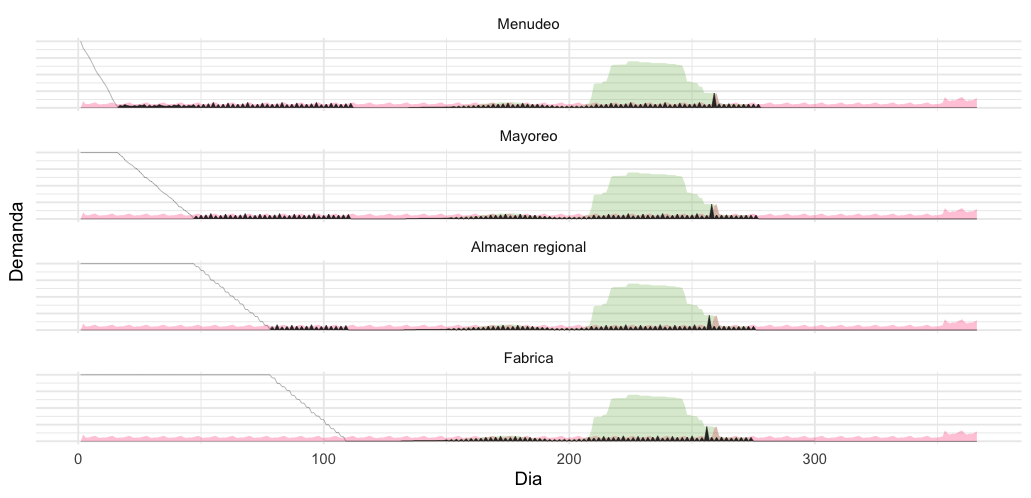
\includegraphics[width=16cm]{tesis_tex/figs/analytic_with_fields_restriction.png}
\centering
\end{figure}

Como se puede observar en la figura \ref{analytic_3}, los agentes no se prepararon adecuadamente para cubrir la demanda posterior al tiempo en que los campos tuvieron producci\'on positiva. Esto sucede porque, en este modelo, los agentes ven solamente un periodo hacia el futuro, as\'i que solo se preparan para ese d\'ia. Esta complicaci\'on vuelve imperante que todos los agentes usen sus almacenes para poder afrontar la demanda, incluso cuando no hay producci\'on. Tal soluci\'on se vuelve compleja porque hay muchos par\'ametros en juego, por mencionar algunos:
\begin{itemize}
    \item El costo diario de almacenamiento influye directamente en qu\'e tanto tiempo un agente puede mantener la cerveza en inventario para cubrir una venta futura, tal que a\'un obtenga un margen positivo cuando \'esta suceda. Si es relevante asegurar que nunca tendr\'an cerveza guardada durante m\'as de un a\~no, o durante cualquier periodo relacionado, por ejemplo, con la caducidad del producto, es necesario que se cumpla la restricci\'on:
    $$
    margen_{agente} <= 365*almacenaje_{agente}
    $$
    \item El castigo por orden no cumplida (\textit{metapolicy}) tambi\'en juega un papel importante en la interacci\'on anterior: si es suficientemente grande, incluso podr\'ia resultar en que un margen negativo causado por el costo de almacenamiento es a\'un preferible a las consecuencias de perder la venta. Si se busca asegurar que siempre sea preferible buscar una venta, es necesario que se cumpla la restricci\'on:
    $$
    castigo_{agente} >= margen_{agente} + 365*almacenaje_{agente}
    $$
    \item Si la producci\'on total en el a\~no es mayor que la demanda total durante el mismo periodo, no es necesario comprarle toda la cebada a los campos. Paralelamente, si la producci\'on es menor a la demanda, es necesario comprar toda la cebada disponible, pues completar algunas ventas siempre es preferible a no completar ninguna
\end{itemize}

Sin embargo, algunas de estas condiciones son te\'oricas y no forzosamente deben cumplirse: es posible que mantener una cerveza en el inventario desde finales de septiembre hasta principios de mayo (cuando vuelve a haber producci\'on) sencillamente no sea redituable. \\

En este trabajo presentaremos un modelo con esta restricci\'on, y lo resolveremos tanto con \textit{policy iteration} como con \textit{Q-learning}. Ambos modelos de aprendizaje reforzado presentados en esta tesis son capaces de capturar todas estas interacciones e incorporarlas al aprendizaje de cada agente.
